\documentclass[a4paper,12pt,twocolumn,landscape]{article}

\usepackage{FabZ}
\usepackage{vecteurs}

\usepackage{geometry}
\geometry{hmargin=0.5cm,vmargin=1.5cm}

%\setlength{\headheight}{0pt}
%\pagestyle{fancyplain}
%\fancyhf{}
%\lhead[]{\textbf{TD Vecteurs}}
%\chead[]{}
%\rhead[]{}
%
%\lfoot[]{}
%\cfoot[]{}
%\rfoot[]{}
%%\rfoot[]{Page \thepage~ sur \pageref{LastPage}}

\fancypagestyle{firststyle}
{
	\setlength{\headheight}{0em}
	\fancyhf{}
	\lhead[]{\textbf{Repérage dans le plan}}
	\chead[]{}
	\rhead[]{\textbf{Repérage dans le plan}}
%	\lhead[]{\textbf{Devoir sur table n°1}}
%	\chead[]{Jeudi 26 septembre 2013}
%	\rhead[]{Géométrie plane, calculs sur les fractions}

	\lfoot[]{}
	\cfoot[]{}
	\rfoot[]{}
%	\rfoot[]{Page \thepage~ sur \pageref{LastPage}}
}

\fancypagestyle{vide}
{
	\setlength{\headheight}{0em}
	\pagestyle{fancyplain}
	\def\headrulewidth{0em}
	\fancyhf{}
	\lhead[]{}
	\chead[]{}
	\rhead[]{}
	
	\lfoot[]{}
	\cfoot[]{}
	\rfoot[]{}
%	\rfoot[]{Page \thepage~ sur \pageref{LastPage}}
}

\usetikzlibrary{fadings}
\newcommand{\Fin}{node[xshift=-1.5ex,rotate=10]{F}
node[rotate=170]{i}
node[xshift=1.5ex,rotate=45]{n}}

\newcommand{\bonnesvacances}{node[xshift=0ex,rotate=10]{B}
node[xshift=1*1.5ex,rotate=170]{o}
node[xshift=2*1.5ex,rotate=45]{n}
node[xshift=3*1.5ex,rotate=128]{n}
node[xshift=4*1.5ex,rotate=75]{e}
node[xshift=5*1.5ex,rotate=130]{s}
node[xshift=6*1.5ex,rotate=85]{~}
node[xshift=7*1.5ex,rotate=128]{v}
node[xshift=8*1.5ex,rotate=43]{a}
node[xshift=9*1.5ex,rotate=4]{c}
node[xshift=10*1.5ex,rotate=145]{a}
node[xshift=11*1.5ex,rotate=5]{n}
node[xshift=12*1.5ex,rotate=25]{c}
node[xshift=13*1.5ex,rotate=105]{e}
node[xshift=14*1.5ex,rotate=45]{s}
}

\begin{document}
\begin{minipage}{0.45\textwidth}
\thispagestyle{firststyle}
%\paragraph*{Exercice}~\\% \hfill \emph{4~points}~\\

\vspace*{2em}

%\input{triangle-milieu-milieu-1}\\

\paragraph{Exercice~3} Copilote

	\begin{center}
	%\fbox{
	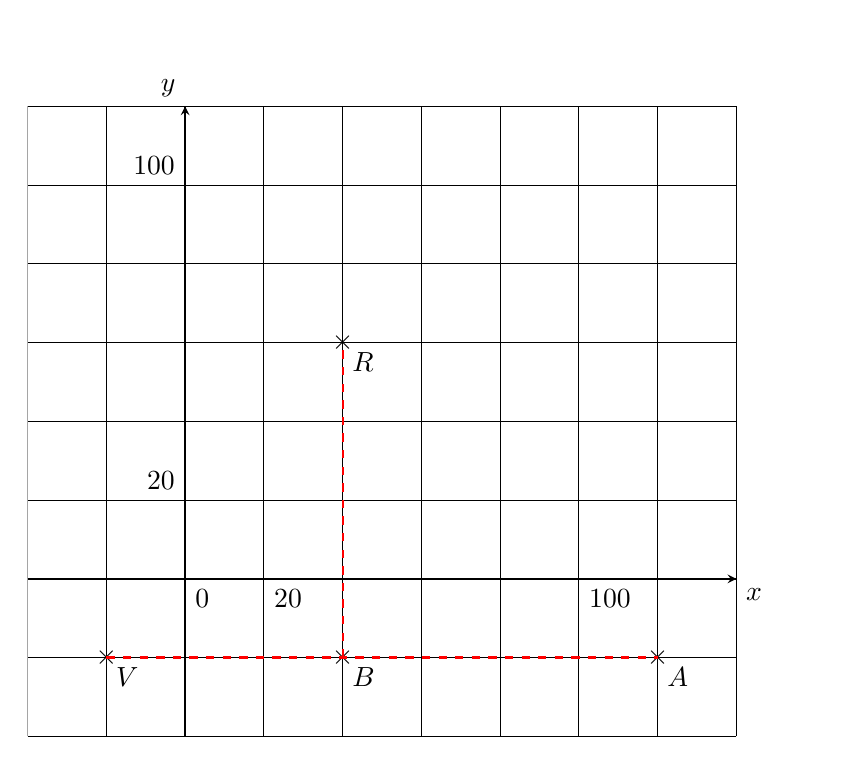
\begin{tikzpicture}[scale=1,every node/.style={scale=1}]
		%Points
		\clip (-2,-2.1) rectangle (8,7);
		\coordinate(O)at(0,0);
		\coordinate(I)at(1,0);
		\coordinate(J)at(0,1);
		\coordinate(xstart)at(-2,0);
		\coordinate(xend)at(7,0);
		\coordinate(ystart)at(0,-2);
		\coordinate(yend)at(0,6);
		\coordinate(V)at(-1,-1);
		\coordinate(B)at(2,-1);
		\coordinate(R)at(2,3);
		\coordinate(A)at(6,-1);
		%Étiquettes
	%	\draw (I) node[below right] {$1$};
	%	\draw (J) node[above left] {$1$};
		\draw (xend) node[below right] {$x$};
		\draw (yend) node[above left] {$y$};
		%%%%%%%%%%%%%%%%%%%%%%%%%%%%%%%%%%%%
		%Axes
		\draw [thick] (xstart) -- (xend);
		\draw [thick] (ystart) -- (yend);
		%Flèches
	%	\draw [>=stealth,->] (O) -- (I);
	%	\draw [>=stealth,->] (O) -- (J);
		\draw [>=stealth,->] (O) -- (xend);
		\draw [>=stealth,->] (O) -- (yend);
		%Grille
		\draw [thin] (-2,-2)grid(7,6);
		%%%%%%%%%%%%%%%%%%%%%%%%%%%%%%%%%%%%
		%étiquettes
		\foreach \point in {V,B,R,A}
			\draw(\point)node{$\times$};
		\foreach \point in {V,B,R,A}
			\draw(\point)node[below right]{$\point$};	
		
    	\draw[thick, below right] (0,0) node{0};
    	\draw[thick, below right] (1,0) node{20};
    	\draw[thick, below right] (5,0) node{100};
    	\draw[thick, above left] (0,1) node{20};
    	\draw[thick, above left] (0,5) node{100};
	    
		\draw [thick,dashed,red] (V) -- (A);
		\draw [thick,dashed,red] (B) -- (R);
		
%		\only<6-|handout:5->{\draw [thick,red] (B) -- (R) node[midway,above,sloped] {$80$};}
%		\only<7-|handout:6->{\draw [thick,green] (V) -- (R) node[midway,above,sloped] {$100$};}
%		\only<4-4|handout:4->{\draw [thick,blue] (V) -- (5,-1) node[near end,below,sloped] {$120$};}
%		\only<4-6|handout:4-5>{\draw [thick,blue] (V) -- (R) node[midway,above,sloped] {$?$};}
%		\only<5-|handout:5->{\draw [thick,red] (V) -- (B) node[midway,below,sloped] {$60$};}
		
	\end{tikzpicture}
	%}
	\\[2em]
	\end{center}
	À quelques kilomètres de l'arrivée d'une course automobile, le véhicule situé en $V$ doit prendre une décision~:\\	
	Peut-il tenter d'aller jusqu'à l'arrivée~$A$ directement ou bien doit-il passer par le ravitaillement~$R$~? Votre rôle de copilote est de l'aider à prendre cette décision.\\ Que lui conseillez-vous ?\\ \textcolor{red}{Il lui reste 120km d'autonomie.}\\
Les points $V$, $R$ et $A$ placés dans le repère orthonormé représentent respectivement les positions de la voiture, du ravitaillement et de l'arrivée.
\vspace{-2em}	

\end{minipage}
\newpage
\begin{minipage}{0.45\textwidth}
\thispagestyle{firststyle}
%\paragraph*{Exercice}~\\% \hfill \emph{4~points}~\\

\vspace*{2em}

%\input{triangle-milieu-milieu-1}\\

\paragraph{Exercice~3} Copilote

	\begin{center}
	%\fbox{
	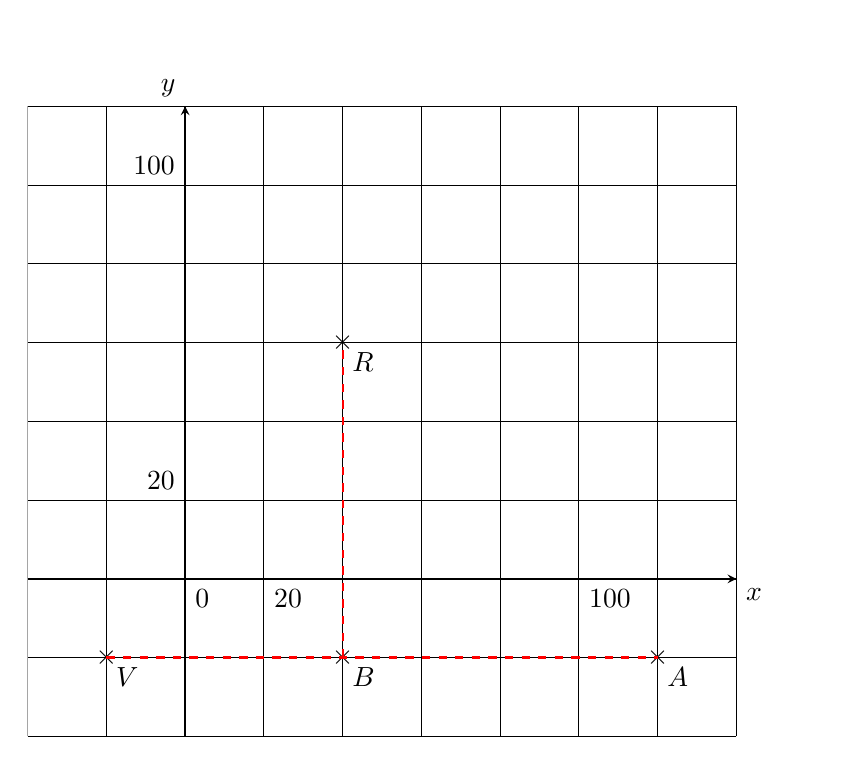
\begin{tikzpicture}[scale=1,every node/.style={scale=1}]
		%Points
		\clip (-2,-2.1) rectangle (8,7);
		\coordinate(O)at(0,0);
		\coordinate(I)at(1,0);
		\coordinate(J)at(0,1);
		\coordinate(xstart)at(-2,0);
		\coordinate(xend)at(7,0);
		\coordinate(ystart)at(0,-2);
		\coordinate(yend)at(0,6);
		\coordinate(V)at(-1,-1);
		\coordinate(B)at(2,-1);
		\coordinate(R)at(2,3);
		\coordinate(A)at(6,-1);
		%Étiquettes
	%	\draw (I) node[below right] {$1$};
	%	\draw (J) node[above left] {$1$};
		\draw (xend) node[below right] {$x$};
		\draw (yend) node[above left] {$y$};
		%%%%%%%%%%%%%%%%%%%%%%%%%%%%%%%%%%%%
		%Axes
		\draw [thick] (xstart) -- (xend);
		\draw [thick] (ystart) -- (yend);
		%Flèches
	%	\draw [>=stealth,->] (O) -- (I);
	%	\draw [>=stealth,->] (O) -- (J);
		\draw [>=stealth,->] (O) -- (xend);
		\draw [>=stealth,->] (O) -- (yend);
		%Grille
		\draw [thin] (-2,-2)grid(7,6);
		%%%%%%%%%%%%%%%%%%%%%%%%%%%%%%%%%%%%
		%étiquettes
		\foreach \point in {V,B,R,A}
			\draw(\point)node{$\times$};
		\foreach \point in {V,B,R,A}
			\draw(\point)node[below right]{$\point$};	
		
    	\draw[thick, below right] (0,0) node{0};
    	\draw[thick, below right] (1,0) node{20};
    	\draw[thick, below right] (5,0) node{100};
    	\draw[thick, above left] (0,1) node{20};
    	\draw[thick, above left] (0,5) node{100};
	    
		\draw [thick,dashed,red] (V) -- (A);
		\draw [thick,dashed,red] (B) -- (R);
		
%		\only<6-|handout:5->{\draw [thick,red] (B) -- (R) node[midway,above,sloped] {$80$};}
%		\only<7-|handout:6->{\draw [thick,green] (V) -- (R) node[midway,above,sloped] {$100$};}
%		\only<4-4|handout:4->{\draw [thick,blue] (V) -- (5,-1) node[near end,below,sloped] {$120$};}
%		\only<4-6|handout:4-5>{\draw [thick,blue] (V) -- (R) node[midway,above,sloped] {$?$};}
%		\only<5-|handout:5->{\draw [thick,red] (V) -- (B) node[midway,below,sloped] {$60$};}
		
	\end{tikzpicture}
	%}
	\\[2em]
	\end{center}
	À quelques kilomètres de l'arrivée d'une course automobile, le véhicule situé en $V$ doit prendre une décision~:\\	
	Peut-il tenter d'aller jusqu'à l'arrivée~$A$ directement ou bien doit-il passer par le ravitaillement~$R$~? Votre rôle de copilote est de l'aider à prendre cette décision.\\ Que lui conseillez-vous ?\\ \textcolor{red}{Il lui reste 120km d'autonomie.}\\
Les points $V$, $R$ et $A$ placés dans le repère orthonormé représentent respectivement les positions de la voiture, du ravitaillement et de l'arrivée.
\vspace{-2em}	

\end{minipage}
\end{document}
